\documentclass[tikz,border=5pt]{standalone}
\usetikzlibrary{angles,quotes,calc,arrows.meta}
\begin{document}

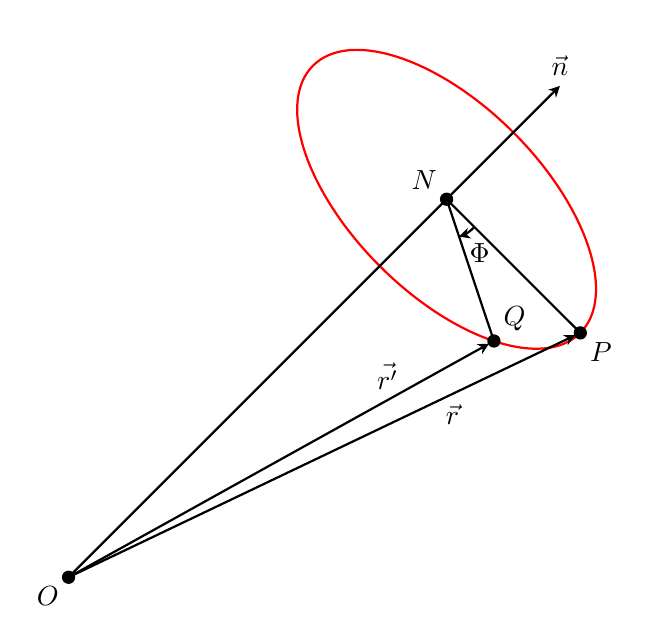
\begin{tikzpicture}[scale=1.2, 
  >={Stealth[length=4pt,width=4pt]},
  vector/.style={->,thick},
  charge/.style={circle,draw,fill=gray!20,minimum size=8pt,inner sep=0pt}
  ]

% Points
\coordinate (O) at (0,0);
\coordinate (N) at (4,4);

% Rotated coordinate system about N
\begin{scope}[rotate around={-45:(N)}]
%Points with rotation
\def\theta{0}
\coordinate (P) at ($(N) + ({2*cos(\theta)},{ sin(\theta)})$);
\def\theta{45}
\coordinate (Q) at ($(N) + ({2*cos(\theta)},{-sin(\theta)})$);
% Ellipse
\draw[thick,red] (N) circle(2cm and 1cm);
\end{scope}
%Edges
\draw[thick] (N) -- (P);
\draw[thick] (N) -- (Q);

% Angle Phi
\pic[<-,draw, thick,"$\Phi$",angle radius=5mm,angle eccentricity=1.6] {angle = Q--N--P};

\draw[->, thick,shorten >=2pt]  (O) -- node[near end, below] {$\vec{r}$} (P);
\draw[->, thick,shorten >=2pt]  (O) -- node[near end, above] {$\vec{r'}$} (Q);
\draw[->, thick]  (O) -- node[at end,above] {$\vec{n}$} (5.2,5.2);
\fill (N) circle (2pt);
\fill (O) circle (2pt);
\fill (P) circle (2pt);
\fill (Q) circle (2pt);
\draw (N) node[above left] {$N$};
\draw (O) node[below left] {$O$};
\draw (P) node[below right] {$P$};
\draw (Q) node[above right] {$Q$};

\end{tikzpicture}

\end{document}